\section{Introduction}

ReScience \sidecite{Rougier:2017} is a peer-reviewed journal that targets
computational research and encourages the explicit replication of already
published research, promoting new and open-source implementations in order to
ensure that the original research is reproducible. The journal has no budget
and is community managed. More specifically, this means there are no production
nor publishing team that could typeset an accepted submission and both authors
and editors are responsible for the final layout of the article. The current
(May 2018) pipeline relies on pandoc \marginnote{\footnotesize Pandoc is a free
  and open-source software document converter, widely used as a writing tool
  and as a basis for publishing
  workflows. \href{https://pandoc.org}{\ExternalLink}} using the markdown
format with a YAML header. The original motivation for using pandoc was first,
to reduce the hassle for the editor and second, to be able to produce an HTML
version of the article. However, experience has proved this was probably a bad
choice and it just made things more difficult for everybody. Pandoc and
asoociated plugins might be difficult to install on some systems and the use of
the markdown markup language severily limits the possibility of the final
layout.\\

The new proposed publishing pipeline is based solely on {\LaTeX } and biber and
aims at facilitating the production and edition of articles.  Since we'll now
directly use {\LaTeX }, this gives us the opportunity to rethink the template.
The proposition (that you're currently reading) is loosely based after
Edward Tufte’s book style where the large left column contains the main text
and the right column is used for auxiliary informations such as notes, captions
or references. Both the style, the layout and the colors of the template aim at
giving ReScience a strong but subtle identity.



% --- Figures -----------------------------------------------------------------
\subsection*{Figures}

There are three styles of figures:
\begin{itemize}
\item Side figure
\item Regular figure
\item Full width figure
\end{itemize}

\marginnote {
  
\begin{tikzpicture}
      \node[draw, fill=black!5, dashed, thick,
            text width=\marginparwidth, minimum height=2.5cm]
            at (0,0) {~~\sf Figure 1};
  \end{tikzpicture}
  \captionof{figure}{Side figure}
  \label{fig:1}
}
Side figures can be easily inserted using:
\begin{lstlisting}
\marginnote
{
  \includegraphics[width=\sidewidth]{...}
  \captionof{figure}{Side figure}
  \label{fig:1}
}
\end{lstlisting}
Result is displayed on figure \ref{fig:1}. This can be used for relatively
small figures and allows to not break the flow of the prose in the document.\\


Regular figures must use the full text width and put the caption in the margin.
Note that you may have to slightly adjust the vertical offset to align caption
and the top of figure which is the recommended layout.\\

\begin{figure}[htbp]
  \marginnote {
    \captionof{figure}{Side caption}
    \label{fig:2}
  }[-2.5em]
  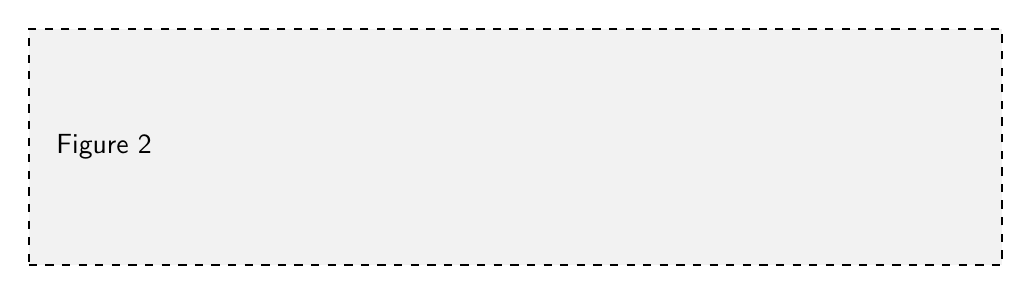
\begin{tikzpicture}
    \node[draw, fill=black!5, dashed, thick,
      text width=\textwidth, minimum height=3cm] at (0,0) {~~\sf Figure 2};
  \end{tikzpicture}
\end{figure}

Corresponding code is:
\begin{lstlisting}
\marginnote
{
  \captionof{figure}{Side caption}
  \label{fig:2}
}[-2.5em]
\includegraphics[width=\textwidth]{...}
\end{lstlisting}

\subsection*{Font stack}
Test
\begin{description}
\item[{\bfseries Serif font}] The
  \href{http://www.tug.dk/FontCatalogue/urwpalladio}{Pazo Math fonts} are a
  family of PostScript fonts suitable for typesetting mathematics in
  combination with the Palatino family of text fonts.
\item[{\sf \bfseries Sans Serif}] The
  \href{http://www.tug.dk/FontCatalogue/firasans/}{Fira Sans fonts} is a
  humanist sans-serif typeface designed by Erik Spiekermann, Ralph du Carrois,
  Anja Meiners and Botio Nikoltchev of Carrois Type Design for the Firefox OS.
\item[{\tt \bfseries Monotype}]
  \href{http://www.tug.dk/FontCatalogue/inconsolata/}{Inconsolata} is
  amonospaced font designed by Raph Levien and has regular and bold weights,
  with additional glyphs and options to control slashed zero, upright quotes
  and a shapelier lower-case L.
\end{description}

An article is composed of four different files:
\begin{lstlisting}
article-metadata.tex
article-header.tex
article-content.tex
article-bibliography.bib
\end{lstlisting}


The {\tt article-metadata.tex} file is generated by the {\tt generate-latex.py}.\\

\begin{minipage}{\fullwidth}
  \em \lipsum[1]
\end{minipage}


%% \marginnote{
%% \begin{figure}[htbp]
%%   \caption{Full width figure ({\tt width=\textbackslash headwidth}) uses a
%%     regular caption}
%%   \label{fig:1}
%% \end{figure}
%% }


%% \begin{figure}[htbp]
%%   \begin{tikzpicture}
%%     \node[draw, fill=black!5, dashed, thick,
%%           text width=.99\headwidth, minimum height=3cm] at (0,0) {~~\sf Figure 3};
%%   \end{tikzpicture}
%%   \marginnote{
%%     \caption{Full width figure using a side caption Lorem ipsum dolor sit amet, consectetuer adipiscing elit.}}[-2.0em]
%%   \label{fig:3}
%% \end{figure}

\section{Commands}

The template defines various commands to help with the writing.
\begin{lstlisting}
\citep{Rougier:2017}\sidecite{Rougier:2017}
\end{lstlisting}

\lipsum[1]

\marginnote{%
  \small
  \begin{tabularx}{\marginparwidth}{lX}
    \bfseries Title 1 & \bfseries Title 2\\
    \hline
    Item 1 & Item 2\\
  \end{tabularx}
  \captionof{table}{Side table}
}

\lipsum[2]
